\begin{figure}
	\centering
	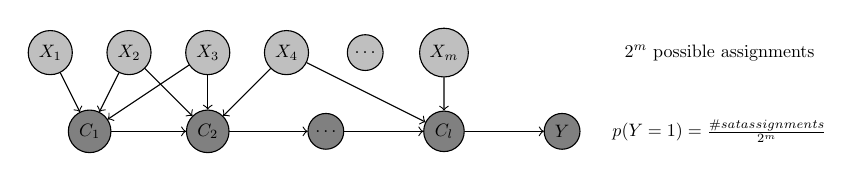
\begin{tikzpicture}[
		scale=0.5,
		every node/.style={scale=0.65},
		clause/.style={circle,draw=black,fill=gray},
		var/.style={circle,draw=black,fill=lightgray}
	]

		% clauses
		\node[clause] (C1) at (0,0) {$C_1$};
		\node[clause] (C2) at (3,0) {$C_2$};
		\node[clause] (dotsC) at (6,0) {$\dots$};
		\node[clause] (Cn) at (9,0) {$C_l$};
		\node[clause] (Y) at (12,0) {$Y$}; \node at (16,0) {$p(Y = 1) = \frac{\text{\# sat assignments}}{2^m}$};

		\draw[->] (C1) -- (C2);
		\draw[->] (C2) -- (dotsC);
		\draw[->] (dotsC) -- (Cn);
		\draw[->] (Cn) -- (Y);

		% variables
		\node[var] (X1) at (-1,2) {$X_1$};
		\node[var] (X2) at (1,2) {$X_2$};
		\node[var] (X3) at (3,2) {$X_3$};
		\node[var] (X4) at (5,2) {$X_4$};
		\node[var] (dotsX) at (7,2) {$\dots$};
		\node[var] (Xm) at (9,2) {$X_m$}; \node at (16,2) {$2^m$ possible assignments};
	
		\draw[->] (X1) -- (C1);
		\draw[->] (X2) -- (C1);
		\draw[->] (X2) -- (C2);
		\draw[->] (X3) -- (C1);
		\draw[->] (X3) -- (C2);	
		\draw[->] (X4) -- (C2);
		\draw[->] (X4) -- (Cn);
		\draw[->] (Xm) -- (Cn);
		
	\end{tikzpicture}
\end{figure}